% Soubory musí být v kódování, které je nastaveno v příkazu \usepackage[...]{inputenc}

\documentclass[             % Základní nastavení
    12pt,       			% Velikost základního písma je 12 bodů
    a4paper,    			% Formát papíru je A4
    oneside,      			% Jednostranný tisk
    unicode,				% Záložky a metainformace ve výsledném  PDF budou v kódování unicode
]{article}				    % Dokument třídy 'zpráva', vhodná pro sazbu závěrečných prací s kapitolami

% ############
% # DŮLEŽITÉ #
% ############

\title{Název dokumentu}                     % Název dokumentu - Povinný
\newcommand{\subtitle}{Popis dokumentu}     % Popis dokumentu - Nepovinný
\author{Czechbol}                           % Autor           - Nepovinný
\newcommand{\grammar}{Czechbol}             % Korektura       - Nepovinný
\newcommand{\formatting}{Czechbol}          % Formátování     - Nepovinný
% ##################
% # PŘIDANÉ BALÍKY #
% ##################

\usepackage[utf8]		    % Kódování zdrojových souborů je UTF-8
	{inputenc}				% Balíček pro nastavení kódování zdrojových souborů

\usepackage[T1]{fontenc}        % nastavení výstupního kódování

\usepackage[				% Nastavení geometrie stránky
	hmargin={25mm,25mm},	% Vnitřní a vnější okraj
	vmargin={25mm,25mm},	% Horní a dolní okraj
	footskip=17mm,			% Velikost zápatí
	nohead,					% Bez záhlaví
]{geometry}

\usepackage{graphicx}           % nutné pro vkládání obrázků
\usepackage[czech]{babel}       % čeština pro LaTeX
\usepackage{sectsty}            % pro nastavení stylu nadpisů
\usepackage{tocloft}
\usepackage[
	breaklinks=true,		    % hypertextové odkazy mohou obsahovat zalomení řádku
	hypertexnames=false         % názvy hypertext. odkazů budou tvořeny nezávisle na názvech TeXu
]{hyperref}                     % balíček 'hyperref' pro sazbu hypertextových odkazů
\usepackage{csquotes}           % automatické sázení uvozovek
\usepackage[bottom]{footmisc}   % vynucení umístění footnotes vespod stránky

\usepackage{caption}            % umožňuje podrobnější nastavení popisků obrázků a výpisů
\usepackage{ifthen}             % if-then-else podmínky (v title)
\usepackage{amsmath}            % balíček pro sazbu náročnější matematiky
\usepackage{amssymb}            % matematické symboly, např. dvojité znaky pomocí \mathbb{} ("Blackboard-Bold")
\usepackage{enumitem}           % pro jednodušší odstranění mezer mezi prvky listu (v itemize)
\usepackage[formats]{listings}	% Balíček pro sazbu zdrojových textů
\usepackage{cmap} 		        % balíček cmap zajišťuje, že PDF vytvořené `pdflatexem' je
											    % plně "prohledávatelné" a "kopírovatelné"
\usepackage{tikz}               % pro vykreslování orientovaných grafů
\usepackage[newfloat]{minted}   % syntax highlighting kódu

% ####################
% # NASTAVENÍ BALÍKŮ #
% ####################
\allsectionsfont{\sffamily}                               % všechny nadpisy bezpatkové
\renewcommand{\cfttoctitlefont}{\Large\bfseries\sffamily} % formát nadpisu v Obsahu
\renewcommand{\cftsubsecdotsep}{\cftdotsep}               % podnadpisy mají tečkované oddělení v obsahu
\hypersetup{                                              % nastavení odkazů
    colorlinks,
    citecolor=black,
    filecolor=black,
    linkcolor=black,
    urlcolor=blue
}
\usetikzlibrary{shapes,arrows}     % tikz rozšíření
\usemintedstyle{pastie}            % nastavení vzhledu syntax highlightingu 
                                        %(musí být odkomentované přidání balíčku minted)

\newenvironment{code}{\captionsetup{type=listing}}{}

% #########
% # START #
% #########

\begin{document}

\SetupFloatingEnvironment{listing}{name=Výpis kódu}

\makeatletter
\begin{titlepage}
    \clearpage
    \vspace*{4cm}
    \begin{center}
    \begin{minipage}{.6\textwidth}
    \begin{center}
    {\Huge \bfseries \sffamily \@title \par}
    \ifthenelse{\equal{\subtitle}{}}        % if \subtitle is empty string,
    {}                                      % nic nepřidávej,
    {                                       % else:
    \vspace{1.5cm}                          % 
    {\Large\itshape  \subtitle \par}         %
    }                                       % konec else bloku
    
    \end{center}
    \end{minipage}
    \end{center}
    \vfill % equivalent to \vspace{\fill}
    % Bottom of the page
	{
	\begin{tabular}{ ll }
        \ifthenelse{\equal{\@author}{}}{}{Text: & \@author}
        \ifthenelse{\equal{\grammar}{}}{}{\\Korektura: & \grammar}
        \ifthenelse{\equal{\formatting}{}}{}{\\Formátování: & \formatting\\}
    \end{tabular}
	} \hfill {\large \today\par}
    \clearpage


\end{titlepage}
\makeatother

\tableofcontents

\section{Lorem ipsum dolor} % Nadpis
Lorem ipsum dolor sit amet, consectetur adipiscing elit. Nullam vehicula vestibulum felis, hendrerit aliquet sapien sodales nec. Phasellus semper quis orci at ultricies. Mauris non magna vitae massa faucibus vestibulum vel id lorem. Vestibulum interdum lobortis nisl, ut rhoncus dui facilisis sed. Donec eget accumsan lectus. Etiam metus leo, tempus vitae velit non, sagittis tempus dui. Vestibulum nec consectetur velit.

\subsection{Podnadpis}
Aenean molestie lectus nec metus consectetur tincidunt. Vivamus volutpat varius nibh, vitae blandit turpis tincidunt nec. Donec a nulla sit amet risus tristique fringilla eu vel magna. Vivamus ultricies finibus erat, nec convallis lorem efficitur id. Nam vitae augue laoreet, rutrum nibh vel, ultrices ante. 

Duis sollicitudin mi sit amet faucibus auctor. Curabitur non erat nibh. Nulla est orci, egestas a risus vel, faucibus finibus nunc. Nullam id arcu a libero bibendum tristique. Aliquam suscipit, velit a rutrum faucibus, purus urna mattis lacus, in sodales risus libero at dolor. Mauris efficitur fringilla metus, at cursus leo porttitor pharetra. Nullam blandit mattis dui, sodales sollicitudin est varius a. Vestibulum erat mauris, consequat vitae laoreet sit amet, sagittis id sem. Ut vel leo facilisis metus efficitur rhoncus ut quis neque. Mauris nisl eros, rutrum ac lectus vitae, condimentum congue leo. Suspendisse mattis urna in dui tristique placerat.

\subsubsection{Podpodnadpis}
Sed euismod dui at est vestibulum rhoncus. Curabitur mattis dui sit amet ligula sagittis bibendum. Fusce aliquam lorem eget mauris ullamcorper ornare. Duis quis arcu sapien. Cras dapibus volutpat dui, at malesuada massa auctor nec. Phasellus turpis quam, varius ac pharetra et, gravida nec ligula. Morbi lobortis elementum nibh, in pharetra dui pulvinar luctus. Fusce convallis dictum tempor.

\vspace{0.5cm} % vertikální odsazení
\noindent Víceúrovňový seznam: 
\begin{itemize}[noitemsep]
    \item Lorem:
    \begin{itemize}[noitemsep]
        \item Lorem ipsum dolor sit
        \item Lorem ipsum dolor sit
        \item Lorem ipsum dolor sit
    \end{itemize}
    \item Ipsum:
    \begin{itemize}[noitemsep]
        \item Lorem ipsum dolor sit
        \item Lorem ipsum dolor sit
        \item Lorem ipsum dolor sit
    \end{itemize}
\end{itemize}

\newpage % konec stránky

\section{Code bloky}
Lorem ipsum dolor sit amet, consectetur adipiscing elit. Nullam vehicula vestibulum felis, hendrerit aliquet sapien sodales nec. Phasellus semper quis orci at ultricies. Mauris non magna vitae massa faucibus vestibulum vel id lorem. Vestibulum interdum lobortis nisl, ut rhoncus dui facilisis sed. Donec eget accumsan lectus. Etiam metus leo, tempus vitae velit non, sagittis tempus dui. Vestibulum nec consectetur velit.

\begin{code} % obal code blocku pro možnost mít pod ním popis
\begin{minted} % code block, mělo by stačit změnit pouze jazyk viz: https://www.overleaf.com/learn/latex/Code_Highlighting_with_minted#Reference_guide
[frame=lines,framesep=2mm,baselinestretch=1.2,fontsize=\footnotesize,linenos]
{python}
import random

from .data import WORDS

class TextLorem():
    def __init__(self, wsep=' ', ssep=' ', psep='\n\n',
                 srange=(4, 8), prange=(5, 10), trange=(3, 6),
                 words=None):
        self._wsep = wsep
        self._ssep = ssep
        self._psep = psep
        self._srange = srange
        self._prange = prange
        self._trange = trange
        if words:
            self._words = words
        else:
            self._words = WORDS

    def sentence(self):
        n = random.randint(*self._srange)
        s = self._wsep.join(self._word() for _ in range(n))
        return s[0].upper() + s[1:] + '.'

    def paragraph(self):
        n = random.randint(*self._prange)
        p = self._ssep.join(self.sentence() for _ in range(n))
        return p

    def text(self):
        n = random.randint(*self._trange)
        t = self._psep.join(self.paragraph() for _ in range(n))
        return t

    def _word(self):
        return random.choice(self._words)
\end{minted}
\caption{Lorem ipsum generátor} % popis code bloku
\label{code:loremipsum}         % pro hyperlinkování
\end{code}

\newpage

\section{Obrázky}

\begin{figure}[h!] % obal pro možnost popisku
\begin{center}     % vycentrování
 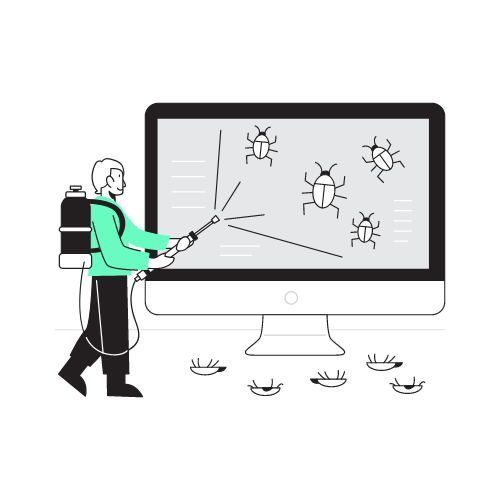
\includegraphics[width=\textwidth]{images/Bug Fixing.png} % vložení obrázku o maximální šířce jako je šířka dokumentu
 \caption{Bug fixing (free to use obrázek z manypixels.co)}   % popis
 \label{img:1}      % odkaz
\end{center}
\end{figure}

\newpage

\vspace{0.5cm}
\begin{figure}[h!]
\begin{center}
\begin{tikzpicture}
  [auto=left,every node/.style={text width=2.5cm,fill=cyan!20},align=center,anchor=west]
  
  \node (A) at (-4.5,4)  {Lorem};
  \node (B) at (0,4)     {Ipsum};
  \node (C) at (0,2)     {Dolor};
  \node (D) at (0,0)     {Sit};
  \node (E) at (4.5,4)   {Amet};
  \node (F) at (4.5,2)   {Consectetur};

  \foreach \from/\to in {A/B,A/C,A/D,B/E,B/F}
    \draw (\from.east) -- (\to.west);
  
\end{tikzpicture}
\caption{Vektorová grafika}
\label{img:2}
\end{center}
\end{figure}


\section{Odkazy}

Je možné používat hypertextové odkazy:

\vspace{0.5cm}
\noindent Pro odkazování v rámci dokumentu slouží label, podívej se znovu na výpis~kódu~\ref{code:loremipsum} a obrázek~\ref{img:1} (klikni na číslo).

\vspace{0.5cm}
\noindent Odkazy na webové stránky:

\noindent For further references see \href{http://www.sharelatex.com}{Something Linky} 
or go to the next url: \url{http://www.sharelatex.com}

\section{Tabulky}

\begin{center}
\begin{tabular}{ c c c }
 cell1 & cell2 & cell3 \\ 
 cell4 & cell5 & cell6 \\  
 cell7 & cell8 & cell9    
\end{tabular}
\end{center}

\begin{center}
\begin{tabular}{ |p{3cm}||p{3cm}|p{3cm}|p{3cm}|  }
 \hline
 \multicolumn{4}{|c|}{Country List} \\
 \hline
 Country Name     or Area Name& ISO ALPHA 2 Code &ISO ALPHA 3 Code&ISO numeric Code\\
 \hline
 Afghanistan   & AF    &AFG&   004\\
 Aland Islands&   AX  & ALA   &248\\
 Albania &AL & ALB&  008\\
 Algeria    &DZ & DZA&  012\\
 American Samoa&   AS  & ASM&016\\
 Andorra& AD  & AND   &020\\
 Angola& AO  & AGO&024\\
 \hline
\end{tabular}
\end{center}

\end{document}
